In the introduction, we showed our choreography language via an
example. We now formalise our language by giving its syntax and
semantics. For the sake of clarity, we slightly change the syntax with
respect to the syntax of our tool.

\mypar{Syntax.} 
%
Let $\role p$ range over a (possibly infinite) set of module names
$\mathcal R$, $x$ over a (possibly infinite) set of variables $\Var$,
and $v$ over a (possibly infinite) set of values $\Val$.
%
Choreographies, the key component of our language, are defined by the
following syntax:
%
\begin{displaymath}\small
  \begin{array}{llllllllllll}
    C \ & ::= & \
      \interact{p}{\role p_1,\ldots,\role p_n}
      \ \mid\
      \ifTE {E}{p}{C_1}{C_2}
      \ \mid\ X \ \mid\  \CEnd
    \\[1mm]
    u     & ::=  & (x' = E)\ \&\ u \quad\mid\quad    (x' = E)
    \qquad\qquad\qquad
    E, g     ::=        f(\tilde E)\quad\mid\quad x\quad\mid\quad v

  \end{array}
\end{displaymath}
% We comment the various constructs.
The syntactic category $C$ denotes choreographic programs. The
interaction term
$\role p\rightarrow \{\role p_1,\ldots,\role
p_n\}:\,\Sigma\{\lambda_j: x_j=E_j.\ C_j\}_{j\in J}$ denotes an
interaction initiated by module $\role p$ with modules $\role p_i$'s
(for $\role p$ and all $\role p_i$ distinct). A choreography specifies
what interaction must be executed next, shifting the focus from what
can happen to what must happen. When the interaction happens, one of
the $j$ branches is selected as a continuation. Branching is a random
move: the number $\lambda_j\in\mathbb R$ denotes either a probability
or a rate. This will depend on the language we wish to use. In the
case of probabilities, it must be the case that $0\leq\lambda_j\leq 1$
and $\Sigma_j\lambda_j=1$. Once a branch $j$ is taken, the
choreography will execute some assignments $u_j$. A single assignment
has the syntax $(x' = E)$ meaning that the value obtained by
evaluating expression $E$ is assigned to variable $x$; assignments can
be concatenated with the operator $\&$.  Note that $x'$ is used for an
assignment to $x$: here, we follow the syntax adopted in PRISM
(see~\S~\ref{sec:prism}). Expressions are obtained by applying some
unspecified functions to other expressions or, as base terms, i.e.,
variables and values (denoted by $v$).
%

The term $\ifTE {E}{p}{C_1}{C_2}$ denotes a system where module
  $\role p$ evaluates the guard $E$ (which can contain variables
  located at other modules) and then (deterministically) branches
  accordingly.  The term $X$ is a (possibly recursive) procedure call:
  in the semantics, we assume that such procedure names are defined
  separately.  The term $\CEnd$ denotes the system finishing its
  computation.

\bigskip


\mypar{Semantics.} In the sequel, we define a state, denoted by $S$,
as a mapping from variables to values, i.e.,
$S: \Var \rightarrow\Val$. Given a value $v$ and a variable $x$, a
substitution $[v/x]$ is an update on a state, i.e.,
$\small S[v/x] (y)= \left\{
  \begin{array}{ll} 
    v    & \text{ if } y=x\\ 
    S(y) & \text{ otherwise}
  \end{array} \right.
$
%
Then, the update $S[u]$ is such that
$S[x'=E\ \&\ u] = S[\eval ES/x][u]$ and $S[x'=E] = S[\eval ES/x]$,
where $\eval ES$ is an unspecified (decidable) evaluation of the
expression $E$ in the state $S$.

Given the set of all possible states $\mathcal S$ and a set of
definitions $\defin$ of the form $X\stackrel{\mathsf{def}}{=} C$, we
can define the operational semantics of choreographies as the minimal
relation
$\red{}\!\!\!\!^\defin\subseteq \mathcal S\times C\times \mathbb
R\times \mathcal S\times C$ such that (we omit $\defin$ if not
relevant):
\begin{displaymath}\small
  \begin{array}{l@{\quad}llll}
    \textsf{(Interact)} &
    (S, \interact{p}{\role p_1,\ldots,\role p_n}) 
    % \red{\Sigma_{(S[u_j],C_j)=(S',C')}\lambda_j}
    % (S', C') 
    \red{\lambda_j}
    (S[u_j], C_j) 
    \\[1mm]
    \textsf{(IfThenElseT)} &
    \eval ES = \mathsf{tt} \quad\Rightarrow\quad
    (S,\ifTE {E}{p}{C_1}{C_2}) 
    \red{1}
    (S, C_1)
    \\[1mm]
    \textsf{(IfThenElseF)} &
    \eval ES = \mathsf{ff} \quad\Rightarrow\quad
    (S,\ifTE {E}{p}{C_1}{C_2}) 
    \red{1}
    (S, C_2)
    \\[1mm]
    \textsf{(Call)} &
    X\stackrel{\mathsf{def}}{=} C\in\defin \quad\Rightarrow\quad (S, X) \red{1}(S,C)
  \end{array}
\end{displaymath}
The transition relation is a Discrete Time Markov Chain (DTMC) or a
Continuous Time Markov Chain (CTMC) depending on whether we use
probabilities or rates in the branching construct. Note that states of
the Markov chain are the pairs $(S,C)$, while the transitions are
given by the relation $\red{}$.
%

% Below, we look at two corner-case examples.
\begin{example}
  Consider the following choreography:
  \begin{displaymath}
    \begin{array}{lll}
      C \ {=}\ \interactBase{p}{q}\ \lambda_1: (x'=1);\quad \interactBase{p}{q}\ \lambda_2: (x'=1);\CEnd
    \end{array}
  \end{displaymath}
  The semantics of $C$ starting from a state in which $S(x)=S(y)=0$
  can be depicted as follows (for
  $C'= \interactBase{p}{q}\ \lambda_1: (x'=1);\CEnd$):

\bigskip
\begin{comment}
\begin{tikzpicture}\small
    \node[state, initial] (1) 
    {\tiny$\begin{array}{c}
      C \\ x=0
    \end{array}$};
    \node[state, right of=1, xshift=3cm] (2) 
        {\tiny$\begin{array}{c}
      C' \\ x=1
    \end{array}$};
    \node[state, right of=2, xshift=3cm] (3) 
        {\tiny$\begin{array}{c}
      \CEnd \\ x=1
    \end{array}$};
     \draw[->]   (1) edge[above] node{$\lambda_1$} (2)
             (2) edge[below] node{$\lambda_2$} (3)
     ;
\end{tikzpicture}
\end{comment}
\begin{figure}[!h]
  \centering
  \vspace{-1cm}
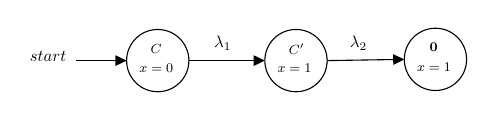
\begin{tikzpicture}[x=0.75pt,y=0.75pt,yscale=-1,xscale=1,scale=0.6, every node/.style={scale=0.6}]
  %uncomment if require: \path (0,300); %set diagram left start at 0, and has height of 300
  %Shape: Circle [id:dp1991798631163264] 
  \draw   (219,126) .. controls (219,112.19) and (230.19,101) .. (244,101) .. controls (257.81,101) and (269,112.19) .. (269,126) .. controls (269,139.81) and (257.81,151) .. (244,151) .. controls (230.19,151) and (219,139.81) .. (219,126) -- cycle ;
  %Shape: Circle [id:dp10467411334622834] 
  \draw   (330,126) .. controls (330,112.19) and (341.19,101) .. (355,101) .. controls (368.81,101) and (380,112.19) .. (380,126) .. controls (380,139.81) and (368.81,151) .. (355,151) .. controls (341.19,151) and (330,139.81) .. (330,126) -- cycle ;
  %Shape: Circle [id:dp3427541367043958] 
  \draw   (442,125) .. controls (442,111.19) and (453.19,100) .. (467,100) .. controls (480.81,100) and (492,111.19) .. (492,125) .. controls (492,138.81) and (480.81,150) .. (467,150) .. controls (453.19,150) and (442,138.81) .. (442,125) -- cycle ;
  %Straight Lines [id:da18643758642972075] 
  \draw    (178,126) -- (216,126) ;
  \draw [shift={(219,126)}, rotate = 180] [fill={rgb, 255:red, 0; green, 0; blue, 0 }  ][line width=0.08]  [draw opacity=0] (8.93,-4.29) -- (0,0) -- (8.93,4.29) -- cycle    ;
  %Straight Lines [id:da45756471809990495] 
  \draw    (269,126) -- (327,126) ;
  \draw [shift={(330,126)}, rotate = 180] [fill={rgb, 255:red, 0; green, 0; blue, 0 }  ][line width=0.08]  [draw opacity=0] (8.93,-4.29) -- (0,0) -- (8.93,4.29) -- cycle    ;
  %Straight Lines [id:da4059508932352085] 
  \draw    (380,126) -- (439,125.05) ;
  \draw [shift={(442,125)}, rotate = 179.08] [fill={rgb, 255:red, 0; green, 0; blue, 0 }  ][line width=0.08]  [draw opacity=0] (8.93,-4.29) -- (0,0) -- (8.93,4.29) -- cycle    ;
  
  % Text Node
  \draw (228,127.4) node [anchor=north west][inner sep=0.75pt]  [font=\footnotesize]  {$x=0$};
  % Text Node
  \draw (237,111.4) node [anchor=north west][inner sep=0.75pt]  [font=\footnotesize]  {$C$};
  % Text Node
  \draw (339,127.4) node [anchor=north west][inner sep=0.75pt]  [font=\footnotesize]  {$x=1$};
  % Text Node
  \draw (348,111.4) node [anchor=north west][inner sep=0.75pt]  [font=\footnotesize]  {$C'$};
  % Text Node
  \draw (451,126.4) node [anchor=north west][inner sep=0.75pt]  [font=\footnotesize]  {$x=1$};
  % Text Node
  \draw (461,110.4) node [anchor=north west][inner sep=0.75pt]  [font=\footnotesize]  {$\mathbf{0}$};
  % Text Node
  \draw (140,117) node [anchor=north west][inner sep=0.75pt]   [align=left] {$\displaystyle start$};
  % Text Node
  \draw (288,105) node [anchor=north west][inner sep=0.75pt]   [align=left] {$\displaystyle \lambda _{1}$};
  % Text Node
  \draw (397,105) node [anchor=north west][inner sep=0.75pt]   [align=left] {$\displaystyle \lambda _{2}$};
  \end{tikzpicture}
  \vspace{-1cm}
\end{figure}
\end{example}


\begin{example}\label{example2}
  Consider the following definition:
  \begin{displaymath}
    \begin{array}{lll}
      C \stackrel{\mathsf{def}}{=} \interactBase{p}{q}
      \left\{
      \begin{array}{lll}
        \lambda_1: (x'=1)\&(y'=2);\ C
        \\
        \lambda_2: (x'=3)\&(y'=1);\ C
      \end{array}
      \right.
    \end{array}
  \end{displaymath}
The semantics of $C$ starting from a state in which $S(x)=S(y)=0$ can
be depicted as follows:

\bigskip
\begin{comment}
\begin{tikzpicture}\small
    \node[state, initial] (1) 
    {\tiny$\begin{array}{c}
      C \\ x=0\\ y=0
    \end{array}$};
    \node[state, right of=1, xshift=4cm] (2) 
        {\tiny$\begin{array}{c}
      C \\ x=1\\ y=2
    \end{array}$};
    \node[state, below right of=1, xshift=1.8cm] (3) 
        {\tiny$\begin{array}{c}
      C \\ x=3\\ y=1
    \end{array}$};
     \draw [->]  (1) edge[above, bend left] node{$\lambda_1$} (2)
             (1) edge[below, bend right] node{$\lambda_2$} (3)
             (2) edge[loop right] node{$\lambda_1$} (2)
             (3) edge[loop below] node{$\lambda_2$} (3)
             (2) edge[below, bend left] node{$\lambda_2$} (3)
             (3) edge[above] node{$\lambda_1$} (2)
     ;
\end{tikzpicture}
\end{comment}
\begin{figure}[h]
  \centering
  \vspace{-1cm}
  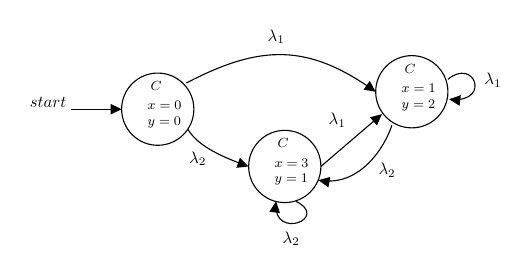
\begin{tikzpicture}[x=0.75pt,y=0.75pt,yscale=-1,xscale=1,scale=0.6, every node/.style={scale=0.6}]
    %uncomment if require: \path (0,448); %set diagram left start at 0, and has height of 448
    %Shape: Circle [id:dp07054898935668796] 
    \draw   (235,148) .. controls (235,131.98) and (247.98,119) .. (264,119) .. controls (280.02,119) and (293,131.98) .. (293,148) .. controls (293,164.02) and (280.02,177) .. (264,177) .. controls (247.98,177) and (235,164.02) .. (235,148) -- cycle ;
    %Straight Lines [id:da7347994961242792] 
    \draw    (194,148) -- (232,148) ;
    \draw [shift={(235,148)}, rotate = 180] [fill={rgb, 255:red, 0; green, 0; blue, 0 }  ][line width=0.08]  [draw opacity=0] (8.93,-4.29) -- (0,0) -- (8.93,4.29) -- cycle    ;
    %Shape: Circle [id:dp22606672052423815] 
    \draw   (337,194) .. controls (337,177.98) and (349.98,165) .. (366,165) .. controls (382.02,165) and (395,177.98) .. (395,194) .. controls (395,210.02) and (382.02,223) .. (366,223) .. controls (349.98,223) and (337,210.02) .. (337,194) -- cycle ;
    %Shape: Circle [id:dp004245899794039332] 
    \draw   (439,134) .. controls (439,117.98) and (451.98,105) .. (468,105) .. controls (484.02,105) and (497,117.98) .. (497,134) .. controls (497,150.02) and (484.02,163) .. (468,163) .. controls (451.98,163) and (439,150.02) .. (439,134) -- cycle ;
    %Curve Lines [id:da36630684284037396] 
    \draw    (287,127) .. controls (347.09,95.48) and (384.85,95.98) .. (436.62,132.31) ;
    \draw [shift={(439,134)}, rotate = 215.64] [fill={rgb, 255:red, 0; green, 0; blue, 0 }  ][line width=0.08]  [draw opacity=0] (8.93,-4.29) -- (0,0) -- (8.93,4.29) -- cycle    ;
    %Curve Lines [id:da4071587559359209] 
    \draw    (288,164) .. controls (293.85,172.78) and (302.55,181.55) .. (334.5,193.11) ;
    \draw [shift={(337,194)}, rotate = 199.44] [fill={rgb, 255:red, 0; green, 0; blue, 0 }  ][line width=0.08]  [draw opacity=0] (8.93,-4.29) -- (0,0) -- (8.93,4.29) -- cycle    ;
    %Straight Lines [id:da7160141088008605] 
    \draw    (395,194) -- (441.72,153.95) ;
    \draw [shift={(444,152)}, rotate = 139.4] [fill={rgb, 255:red, 0; green, 0; blue, 0 }  ][line width=0.08]  [draw opacity=0] (8.93,-4.29) -- (0,0) -- (8.93,4.29) -- cycle    ;
    %Curve Lines [id:da7788168425777569] 
    \draw    (452,161) .. controls (446.18,178.46) and (427.19,209.09) .. (395.93,205.44) ;
    \draw [shift={(393,205)}, rotate = 10.3] [fill={rgb, 255:red, 0; green, 0; blue, 0 }  ][line width=0.08]  [draw opacity=0] (8.93,-4.29) -- (0,0) -- (8.93,4.29) -- cycle    ;
    %Curve Lines [id:da05888759989591952] 
    \draw    (375,222) .. controls (402.16,235.58) and (357.81,252.92) .. (358.78,224.75) ;
    \draw [shift={(359,222)}, rotate = 97.13] [fill={rgb, 255:red, 0; green, 0; blue, 0 }  ][line width=0.08]  [draw opacity=0] (8.93,-4.29) -- (0,0) -- (8.93,4.29) -- cycle    ;
    %Curve Lines [id:da66106493809224] 
    \draw    (497,124) .. controls (518.34,106.54) and (531.21,141.77) .. (500.93,140.25) ;
    \draw [shift={(498,140)}, rotate = 6.71] [fill={rgb, 255:red, 0; green, 0; blue, 0 }  ][line width=0.08]  [draw opacity=0] (8.93,-4.29) -- (0,0) -- (8.93,4.29) -- cycle    ;
    
    % Text Node
    \draw (248,138.4) node [anchor=north west][inner sep=0.75pt]  [font=\footnotesize]  {$ \begin{array}{l}
    x=0\\
    y=0
    \end{array}$};
    % Text Node
    \draw (257,124.4) node [anchor=north west][inner sep=0.75pt]  [font=\footnotesize]  {$C$};
    % Text Node
    \draw (160,137) node [anchor=north west][inner sep=0.75pt]   [align=left] {$\displaystyle start$};
    % Text Node
    \draw (350,184.4) node [anchor=north west][inner sep=0.75pt]  [font=\footnotesize]  {$ \begin{array}{l}
    x=3\\
    y=1
    \end{array}$};
    % Text Node
    \draw (359,170.4) node [anchor=north west][inner sep=0.75pt]  [font=\footnotesize]  {$C$};
    % Text Node
    \draw (452,124.4) node [anchor=north west][inner sep=0.75pt]  [font=\footnotesize]  {$ \begin{array}{l}
    x=1\\
    y=2
    \end{array}$};
    % Text Node
    \draw (461,110.4) node [anchor=north west][inner sep=0.75pt]  [font=\footnotesize]  {$C$};
    % Text Node
    \draw (351,83) node [anchor=north west][inner sep=0.75pt]   [align=left] {$\displaystyle \lambda _{1}$};
    % Text Node
    \draw (400,150) node [anchor=north west][inner sep=0.75pt]   [align=left] {$\displaystyle \lambda _{1}$};
    % Text Node
    \draw (525,118) node [anchor=north west][inner sep=0.75pt]   [align=left] {$\displaystyle \lambda _{1}$};
    % Text Node
    \draw (288,181) node [anchor=north west][inner sep=0.75pt]   [align=left] {$\displaystyle \lambda _{2}$};
    % Text Node
    \draw (440,190) node [anchor=north west][inner sep=0.75pt]   [align=left] {$\displaystyle \lambda _{2}$};
    % Text Node
    \draw (363,245) node [anchor=north west][inner sep=0.75pt]   [align=left] {$\displaystyle \lambda _{2}$};
    
    
    \end{tikzpicture}
  \vspace{-1cm}
  \end{figure}
\end{example}

%%% Local Variables: 
%%% mode: latex
%%% TeX-master: "main"
%%% End:
